\chapter{Computational Photography}

Data recorded by sensor is not the final image. Computational Photography: arbitrary computation to the final image. 

\section{High Dynamic Range Imaging (HDR)}
高动态范围成像

\begin{figure}[H]
    \centering
    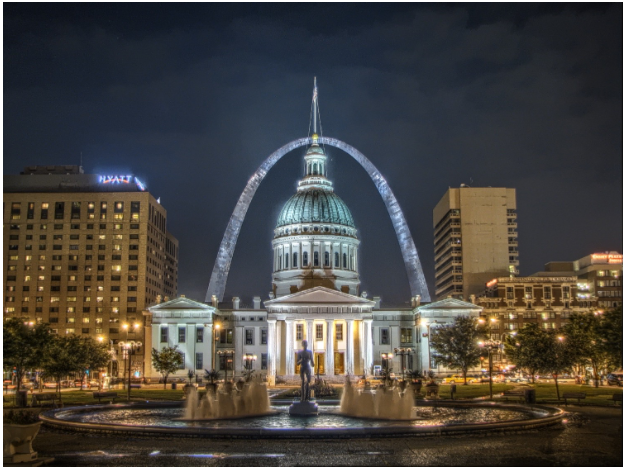
\includegraphics[width=0.209\textwidth]{Lec12/HDR}
    \caption{HDR}
\end{figure}

\subsection{Exposure}
Roughly speaking, the “brightness” of a captured image given a fixed scene.

Exposure = Gain(增益) x Irradiance x Time

Gain is controlled by the ISO. Irradiance is controlled by the aperture. Time is controlled by the shutter speed. 

\subsubsection{shutter speed}
Side-effects of shutter speed: moving scene elements appear blurry. 

\begin{figure}[H]
    \centering
    \begin{subfigure}{0.309\textwidth}
        \centering
        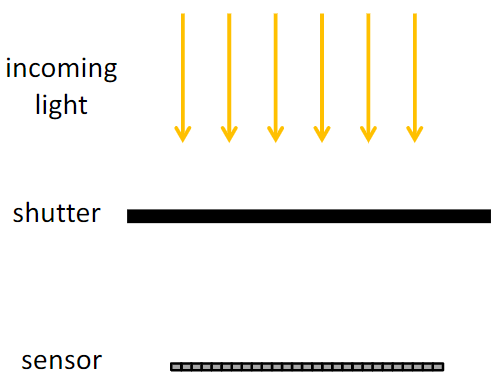
\includegraphics[width=\textwidth]{Lec12/shutter speed close}
        \caption{shutter speed close}
    \end{subfigure}
    \begin{subfigure}{0.309\textwidth}
        \centering
        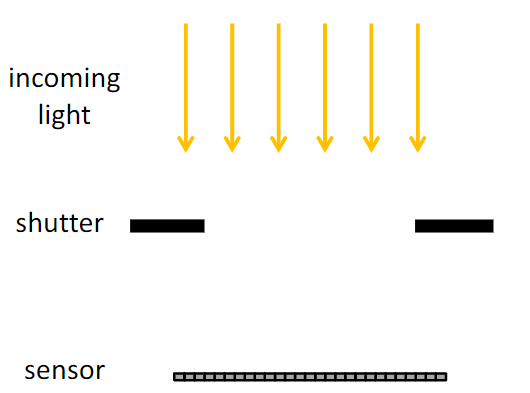
\includegraphics[width=\textwidth]{Lec12/shutter speed open}
        \caption{shutter speed open}
    \end{subfigure}
    \caption{shutter speed}
\end{figure}


\subsubsection{aperture}
Side-effects of aperture: depth of field (bokeh)

\begin{figure}[H]
    \centering
    \begin{subfigure}{0.618\textwidth}
        \centering
        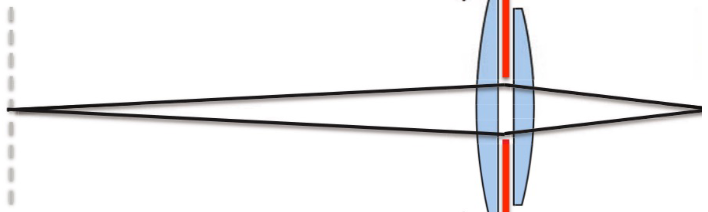
\includegraphics[width=\textwidth]{Lec12/small aperture}
        \caption{small aperture}
    \end{subfigure}

    \begin{subfigure}{0.618\textwidth}
        \centering
        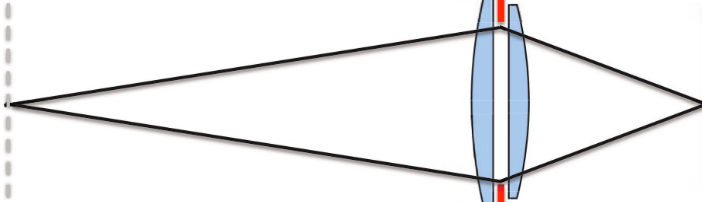
\includegraphics[width=\textwidth]{Lec12/big aperture}
        \caption{big aperture}
    \end{subfigure}
    \caption{aperture}
\end{figure}

\subsubsection{ISO}
ISO 越大图越亮, 但噪声也越多. 

When taking a photo, the averaged exposure should be at the middle of the sensor’s measurement range. So that the photo has both bright and dark parts with details.


\subsection{Dynamic range}
The ratio between the largest and smallest values of a certain quantity (e.g., brightness). 

\begin{figure}[H]
    \centering
    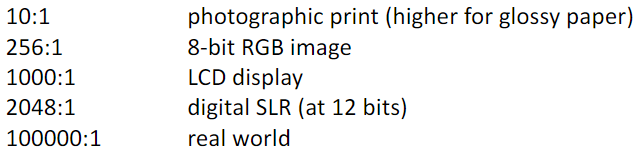
\includegraphics[width=0.668\textwidth]{Lec12/Dynamic range}
    \caption{Dynamic range}
\end{figure}

\subsection{Key idea}
\begin{enumerate}
    \item Exposure bracketing: Capture multiple LDR images at different exposures. 
    \item Merging: Combine them into a single HDR image. 
\end{enumerate}


\subsubsection{Image formation model}
Suppose scene radiance for image pixel $(x, y)$ is $L(x, y)$. 
\begin{align*}
    I(x,y)=clip\left[ t_i\cdot L(x,y)+noise \right]
\end{align*}
clip截断超过相机的数值. Exposure time is $t_i$. 

\begin{figure}[H]
    \centering
    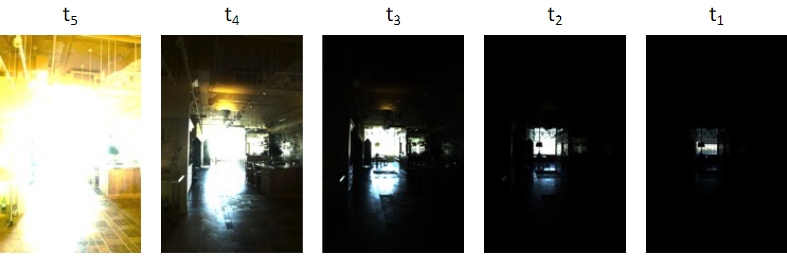
\includegraphics[width=0.618\textwidth]{Lec12/Exposure time}
    \caption{Exposure time}
\end{figure}



\subsubsection{Merging images}
For each pixel:
\begin{enumerate}
    \item Find “valid” pixels in each image. 
    \begin{align*}
        (\text{noise})0.05<\text{pixel}<0.95(\text{clipping})
    \end{align*}
    \item Weight valid pixel values appropriately. 
    \begin{align*}
        \text{weight}=\frac{\text{pixel value}}{t_i}
    \end{align*}
    \item Form a new pixel value as the weighted average of valid pixel values
\end{enumerate}

\subsubsection{Merging result}

\begin{figure}[H]
    \centering
    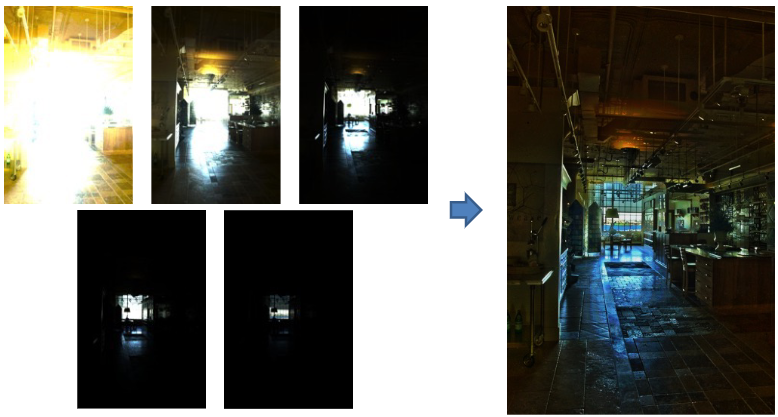
\includegraphics[width=0.618\textwidth]{Lec12/Merging result}
    \caption{Merging result}
\end{figure}

\subsection{Display the HDR image}
how to display the HDR image (e.g. 12-bit) on a SDR(standard dynamic range, e.g., 8-bit) device? tone mapping. 

\subsubsection{Tone mapping}

\begin{figure}[H]
    \centering
    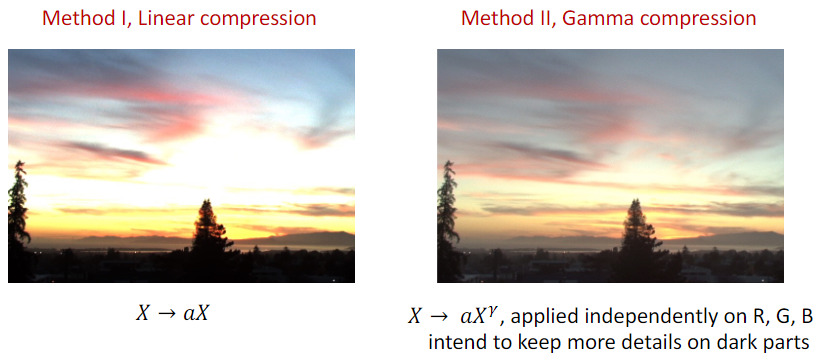
\includegraphics[width=0.618\textwidth]{Lec12/Tone mapping}
    \caption{Tone mapping}
\end{figure}

Gamma compression:$y=ax^{\gamma}$

\begin{figure}[H]
    \centering
    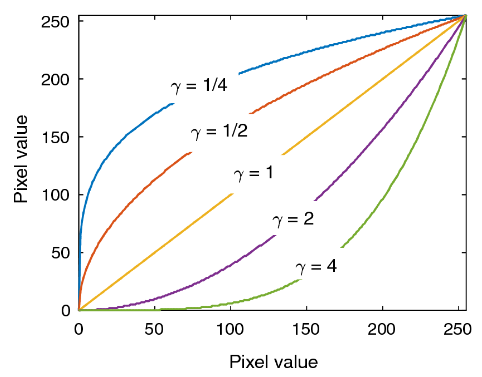
\includegraphics[width=0.618\textwidth]{Lec12/Gamma compression}
    \caption{Gamma compression}
\end{figure}

\section{Deblurring}
\subsection{Reason of blurring}
\begin{itemize}
    \item Defocus: the subject is not in the depth of view. 
    \item Motion blur: moving subjects or unstable camera. 
\end{itemize}

\begin{figure}[H]
    \centering
    \begin{subfigure}{0.309\textwidth}
        \centering
        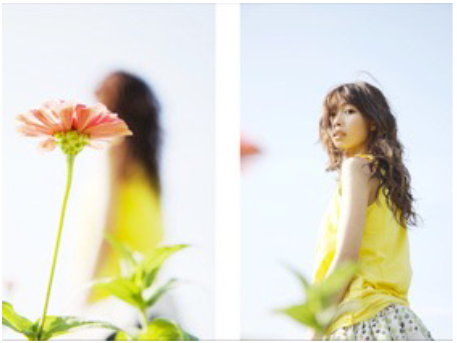
\includegraphics[width=\textwidth]{Lec12/Defocus}
        \caption{Defocus}
    \end{subfigure}
    \begin{subfigure}{0.309\textwidth}
        \centering
        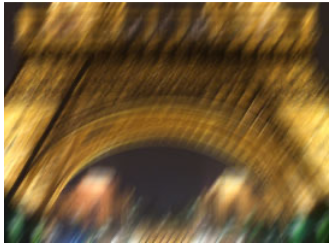
\includegraphics[width=\textwidth]{Lec12/Motion blur}
        \caption{Motion blur}
    \end{subfigure}
    \caption{Blurring}
\end{figure}

\subsection{Get a clear image}
Accurate focus, Fast shutter speed
\begin{itemize}
    \item Large aperture
    \item High ISO
\end{itemize}
One of the reasons why SLR cameras and lenses are expensive. 
\begin{enumerate}
    \item Use hardware
    \begin{itemize}
        \item tripod
        \item not portable!
    \end{itemize}
    \item Use hardware
    \begin{itemize}
        \item optical image stabilization
        \item IMU
        \item expensive!
    \end{itemize}
\end{enumerate}

\subsection{Modeling image blur}
The blurring process can be described by convolution. The blurred image is called convolution kernel. 

\begin{figure}[H]
    \centering
    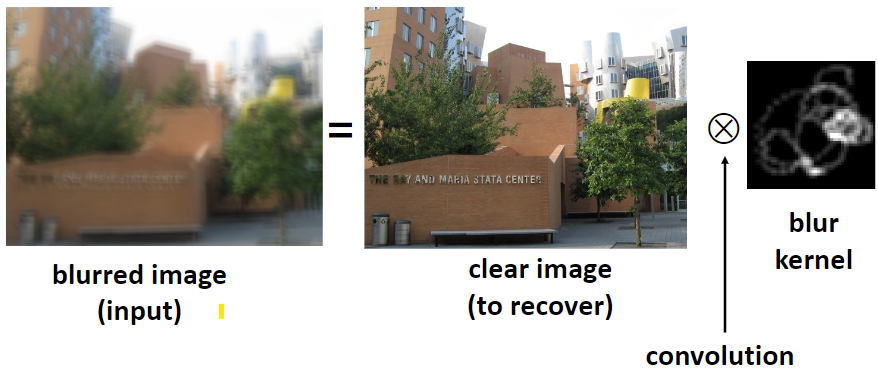
\includegraphics[width=0.618\textwidth]{Lec12/Modeling image blur}
    \caption{Modeling image blur}
\end{figure}

The blur pattern of defocusing depends on the aperture shape. 
The blur pattern of shaking depends on the camera trajectory. 

\begin{align*}
    \text{Deblurring} = \text{Deconvolution}
\end{align*}

\subsection{Non-blind image deconvolution(NBID)}
\begin{align*}
    G=F\bigotimes H
\end{align*}
\begin{itemize}
    \item G: The captured image (known)
    \item F: Image to be solved (unknown)
    \item H: Convolution kernel (known)
\end{itemize}

\subsubsection{Frequency domain deconvolution}
Convolution in the spatial domain = product in the frequency domain. 

\begin{align*}
    \mathcal{F} (G)=\mathcal{F}(F\bigotimes H)=\mathcal{F}(F)\times \mathcal{F}(H)
\end{align*}

Spatial deconvolution = division in frequency domain. 

\begin{align*}
    F=\mathcal{F}^{-1}\left( \mathcal{F}(G) \div \mathcal{F}(H) \right)
\end{align*}

Usually called inverse filter Inverse filter. 

\begin{figure}[H]
    \centering
    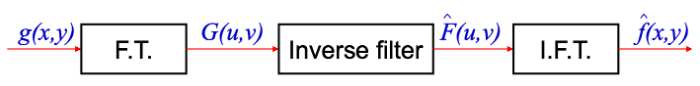
\includegraphics[width=0.618\textwidth]{Lec12/Inverse filter}
    \caption{Inverse filter}
\end{figure}

(但是因为危险的除法)

The blurred kernel is generally a low-pass filter. Inverse filter will amplify high frequency components. Inverse filter will also amplify noise. 
\begin{align*}
    G(u,v)=&H(u,v)F(u,v)+N(u,v)\\
    \hat{F}(u,v)=&\frac{G(u,v)}{H(u,v)}=F(u,v)+\frac{N(u,v)}{H(u,v)}
\end{align*}

\subsubsection{Wiener Filter}
Suppress high frequency when reverse filtering
\begin{align*}
    \hat{F}(u,v)=&W(u,v)G(u,v)\\
    W(u,v)=&\frac{H^*(u,v)}{\left|H(u,v)\right|^2+K(u,v)}
\end{align*}

\begin{itemize}
    \item If $K=0$ then $W(u,v)=\frac{1}{H(u,v)}$, i.e. an inverse filter. 
    \item If $K \gg \left|H(u,v)\right|$ for large $u,v$, then high frequencies are attenuated. 
    \item $K$ is set to a constant scalar which is determined empirically. 
\end{itemize}

\subsubsection{Deconvolution by optimization}
Blurred image generation process:
\begin{align*}
    G=F \bigotimes H+N
\end{align*}

Assuming that the noise $N$ is Gaussian noise, the
likelihood can be measured by the mean square error:
\begin{align*}
    MSE=\left\| G-F \bigotimes H \right\|_2^2=\sum_{ij}\left( G_{ij}-\left[ F \bigotimes H \right]_{ij} \right)^2
\end{align*}

But deconvolution is ill-posed, non-unique solution. Need prior information about the solution. 

Prior of natural image: 
\begin{enumerate}
    \item Natural images are generally smooth in segments
    \item Gradient map is sparse
    \item Adding L1 regularization makes the image gradient sparse. 
\end{enumerate}

Objective function = likelihood function + regular term
\begin{align*}
    \min_F\left\| G-F \bigotimes H \right\|_2^2+\left\| \nabla F \right\|_1
\end{align*}

\subsection{Blind image deconvolution(BID)}
The convolution kernel is also unknown. Obviously more difficult. Need more prior knowledge!

\subsubsection{Kernel prior}
Blur kernel is non-negative and sparse. Optimized objective function:
\begin{align*}
    &\min_F\left\| G-F \bigotimes H \right\|_2^2+ \lambda_1 \left\| \nabla F \right\|_1+\lambda_2 \left\| H \right\|_1\\
    &s.t.H\ge 0
\end{align*}

\section{Colorization}
Colorization refers to the process of adding color to a monochrome picture or video with the aid of a computer. There are two main ways to color grayscale images: 
\begin{enumerate}
    \item Sample-based colorization: use sample image. 
    \item Interactive colorization: paint brush interactively. 
\end{enumerate}

\subsection{Sample-based colorization}

\begin{figure}[H]
    \centering
    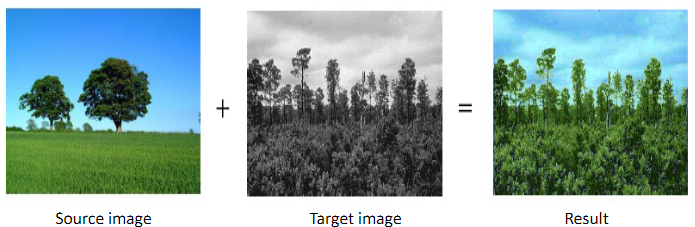
\includegraphics[width=0.618\textwidth]{Lec12/Sample-based colorization}
    \caption{Sample-based colorization}
\end{figure}

Scan the target image, for each pixel:
\begin{enumerate}
    \item Find the best matching point in the sample (e.g. considering the brightness and the standard deviation with neighboring pixels)
    \item Assign the color of the matching point to the pixel
\end{enumerate}

\subsection{Interactive colorization}

\begin{figure}[H]
    \centering
    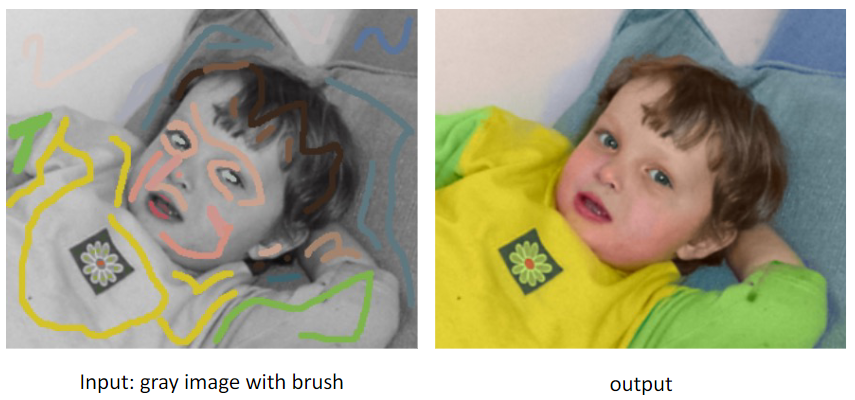
\includegraphics[width=0.618\textwidth]{Lec12/Interactive colorization}
    \caption{Interactive colorization}
\end{figure}

For two adjacent pixels, if the brightness is similar, then the
color should also remain similar. Based on this assumption, the coloring problem is transformed into an optimization problem:
\begin{align*}
    J(U)=\sum_r \left( U(r)-\sum_{s\in N(r)}w_{rs}U(s) \right)^2
\end{align*}

\begin{itemize}
    \item $U(r), U(s)$: RGB values of pixel $r, s$. 
    \item $N(r)$: neighborhood pixels of pixel $r$.  
    \item $w_{rs}$: Weight that measures similarity between $r$ and $s$. 
\end{itemize}

Constraint: User-specified colors of brushed pixels keep unchanged. 

\subsection{The modern approach}
\begin{figure}[H]
    \centering
    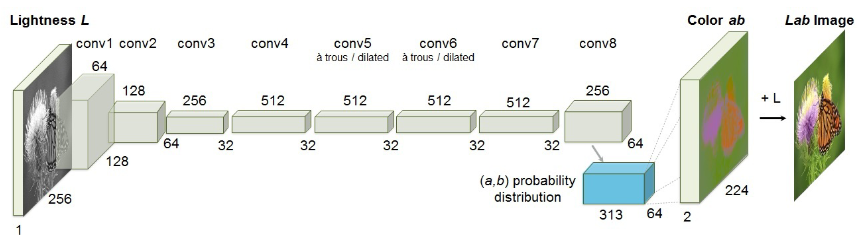
\includegraphics[width=0.618\textwidth]{Lec12/Convolutional Neural Networks}
    \caption{Convolutional Neural Networks}
\end{figure}

\subsubsection{Loss function for image synthesis}
Reconstruction loss: 
\begin{align*}
    L(\Theta )=\left\| F(X;\Theta)-Y \right\|^2
\end{align*}

Problem with reconstruction loss: 
\begin{itemize}
    \item Cannot handle the case with multiple
    solutions
    \item Cannot measure if an image is
    realistic
\end{itemize}

\subsubsection{Generative Adversarial Network (GAN)}
\begin{figure}[H]
    \centering
    \begin{subfigure}{0.618\textwidth}
        \centering
        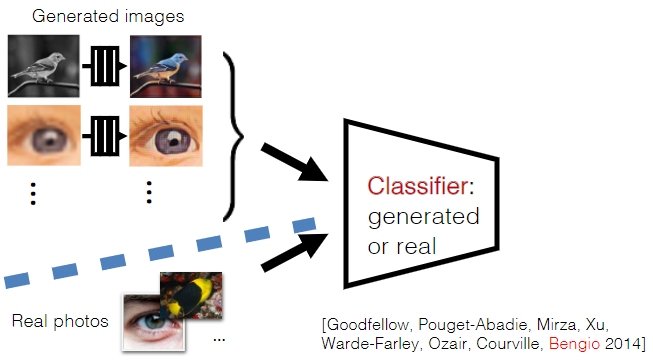
\includegraphics[width=\textwidth]{Lec12/GAN}
    \end{subfigure}

    \begin{subfigure}{0.618\textwidth}
        \centering
        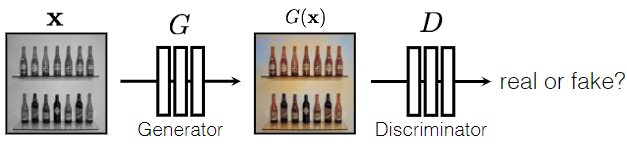
\includegraphics[width=\textwidth]{Lec12/GAN2}
    \end{subfigure}
    \caption{GAN}
\end{figure}

\textbf{G} tries to synthesize fake images that fool \textbf{D}. \textbf{D} tries to identify the fakes. 

Training discriminator: 

\begin{figure}[H]
    \centering
    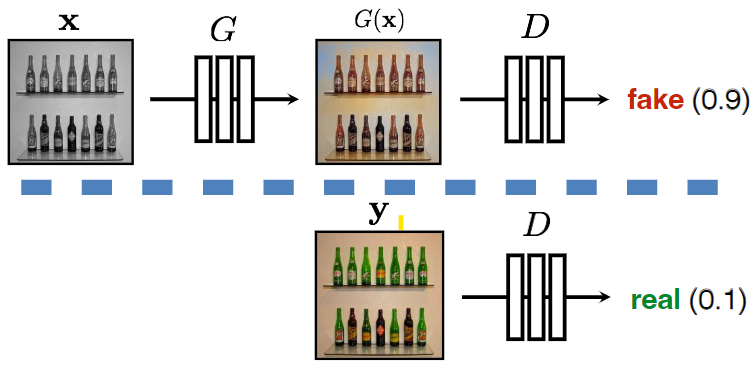
\includegraphics[width=0.618\textwidth]{Lec12/Training discriminator}
    \caption{Training discriminator}
\end{figure}

\begin{align*}
    \arg \max_D \mathbb{E}_{\mathbf{x,y}}\left[ \log D(G(\mathbf{x}))+\log (1-D(\mathbf{y})) \right]
\end{align*}

Training generator: 

\begin{figure}[H]
    \centering
    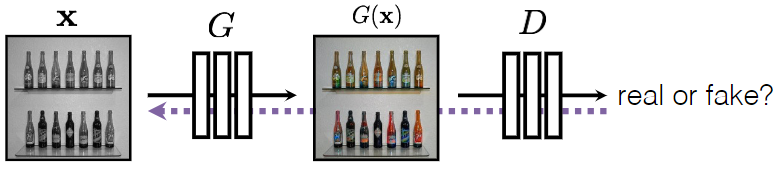
\includegraphics[width=0.618\textwidth]{Lec12/Training generator}
    \caption{Training generator}
\end{figure}

\textbf{G} tries to synthesize fake images that \textcolor{light_red}{fool} \textbf{D}: 

\begin{align*}
    \arg \min_G \mathbb{E}_{\mathbf{x,y}}\left[ \log D(G(\mathbf{x})) \right]
\end{align*}

But for true, we training both of them together: 

\begin{figure}[H]
    \centering
    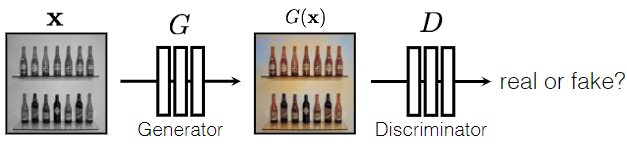
\includegraphics[width=0.618\textwidth]{Lec12/GAN2}
    \caption{Training}
\end{figure}

\textbf{G} tries to synthesize fake images that \textcolor{light_red}{fool} the \textcolor{light_blue}{best} \textbf{D}:

\begin{align*}
    \arg \min_G \max_D \mathbb{E}_{\mathbf{x,y}}\left[ \log D(G(\mathbf{x}))+\log (1-D(\mathbf{y})) \right]
\end{align*}

GAN很难调, 难以收敛. 最近的vae与diffusion model缓解GAN的训练问题. 以及GAN的改进Cycle-GAN, 解决了缺少成对训练数据的问题. 

\begin{figure}[H]
    \centering
    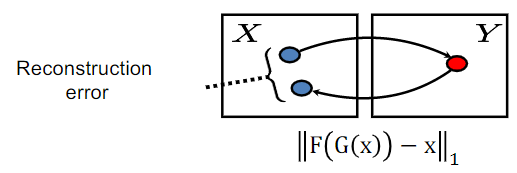
\includegraphics[width=0.618\textwidth]{Lec12/Cycle-GAN}
    \caption{Cycle-GAN}
\end{figure}


\textbf{D} can be viewed as a loss function to train G, called \textcolor{light_red}{adversarial loss}. 
\begin{itemize}
    \item Learned instead of being hand-designed. 
    \item Can be applied to any image synthesis task. 
\end{itemize}

\subsection{More image sysnthesis tasks}
\begin{itemize}
    \item Image to Image Translation. 
    \item Style transfer. 
    \item Text-to-Photo. 
    \item Image dehazing. 
    \item Customized gaming. 
\end{itemize}

\section{Super Resolution}

\subsection{Super Resolution using GAN}

\begin{figure}[H]
    \centering
    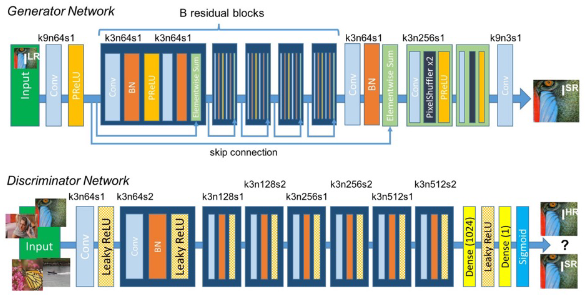
\includegraphics[width=0.518\textwidth]{Lec12/Super Resolution using GAN}
    % \caption{Super Resolution using GAN}
\end{figure}

\begin{figure}[H]
    \centering
    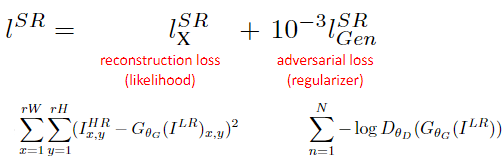
\includegraphics[width=0.418\textwidth]{Lec12/GANGAN}
    \caption{Super Resolution using GAN}
\end{figure}
